%TODO think about the naming
\chapter{Prominent Claim Identification}

Prominent claim identification aims to determine which claims are predominately
used to express and base users' stance on. The task of prominent claim
identification has also been reffered to as \textit{argument-based opinion mining}
\citep{boltuzic2014back}, reason classification \citep{hasan2014you}, and
argument tagging \citep{sobhani2015argumentation}. 
The problem of prominent claim identification involves determining
the relationship between a comment a set of well-established prominent claims. 
Consider a discussion on the topic ``\emph{Should gay marriage be legal}''
and a following comment: 
\begin{quote}
\emph{
Gay marriages must be legal in all 50 states. A marriage is covenant
between 2 people regardless of their genders. Discrimination against
gay marriage is unconstitutional and biased. Tolerance,education and
social justice make our world a better place.
}
\end{quote}
This comment supports the claim ``\emph{It is discriminatory to refuse
gay couples the right to marry}'' and attacks the claim
``\emph{Marriage should be between a man and a woman}''. 
The technical challenge here lies in the fact that, unlike
in debates or other more formal, argumentation sources, 
claims provided by users are usually less formal, ambiguous, vague, 
implicit, or often simply poorly worded. 
The task of \textbf{prominent claim identification} is defined 
as identifying what prominent claims, from a predefined set of prominent claims, 
have been used in users' comments, and how. 
A topic-dependent set of prominent claims is assumed to exist. 
Users' comments typically contain more than one claim, but in their 
own wording and with varying degree of explicitness. 
The task of prominent claim identification amounts to matching
users' comments to prominent claims, which can be either attack or 
supported by the comment. 
The user comment may be a single prominent claim (and it often is), but it 
is reffered to as a \textit{comment} to emphasize the fact that in general 
it may contain several claims, as well as non-argumentative text. 

In this chapter, we first introduce the \ComArg corpus in section~\ref{sec:comarg}
which contains labelled pairs of comments with prominent claims. Next, 
we build a model for prominent claim identification as described in 
section~\ref{sec:argrec_model}. The model is evaluated in 
section~\ref{sec:argrec_experiments}. Finally, we conclude in 
section~\ref{sec:argrec_conclusion}.

\begin{table}
\centering
{\small
\begin{tabular}{cl}
\toprule
Label & Description: Comment\dots \\
\midrule
\textbf{A} & \dots explicitly \textbf{attacks} the prominent claim \\
\textbf{a} & \dots vaguely/implicitly \textbf{attacks} the prominent claim \\
\textbf{N} & \dots makes \textbf{no use} of the prominent claim \\
\textbf{s} & \dots vaguely/implicitly \textbf{supports} the prominent claim \\
\textbf{S} & \dots explicitly \textbf{supports} the prominent claim \\
\bottomrule
\end{tabular}
}
\caption{Labels for comment-prominent claim pairs in the \ComArg corpus}
\label{tab:comarg-labels}
\end{table}

\section{\ComArg corpus}
\label{sec:comarg}

- For training and evaluating argument recognition models,
we have compiled a corpus of user comments, manually annotated
with arguments which we refer to as \ComArg \\
- \ComArg is freely available
\footnote{Freely available under the CC BY-SA-NC license from \url{http://takelab.fer.hr/data/comarg}} \\
- as a source of data we use two websites: 
\emph{procon.org}\footnote{\url{http://www.procon.org}} and 
\textit{idebate.org}.\footnote{\url{http://idebate.org}} \\
The former is a discussion site covering ideological, social, political,
and other topics \\
- users express their personal opinions on a selected topic, taking either
the pro or con side. \\
The latter, \textit{idebate.org} is a debating website containing
online debates and an archive of past debates \\
- each archived topic contains a set of prominent claims 
presented in the debate \\
- each claim is labelled as either \textbf{for} or \textbf{against} the topic \\
- the claims are moderated and edited to provide the best quality of information \\

\noindent two datasources are completentary to each other as 
\textit{procon.org} contains user comments, while \textit{idebate.org} contains prominent 
claims \\
- we manually identified near-identical topics covered by both web sites \\
- we choose two topics: ``\textit{Under God in Pledge}'' (UGIP) and 
``\textit{Gay marriage}'' (GM). \\
- they have a larger-than-average number of comments (above 300) and are 
well-balanced between \textbf{pro} and \textbf{con} stances \\
- for these two topics, we then took the corresponding comments and prominent claims
from \textit{procon.org} and \textit{idebate.org} respectively \\
- as the users can produce comments not relevant to the topic, we skim-read 
the comments and omit non-argumentative comments \\
- we end up with a set of 175 comments and 6 arguments for UGIP, and 198 comments and 7 
arguments for the GM topic \\
- the comments are often verbose: the average number of words per comment is 116 \\
- each comment has an associated stance (\textbf{pro} or \textbf{con}) depending on 
how it was classified in \textit{procon.org} \\
- similarly, each prominent claim either attacks or supports the claim of the topic,
depending on how it was classified on \textit{idebate.org}, these claims will be reffered to 
as ``pro prominent claims'' and ``con prominent claims'' \\
- table~\ref{tab:comarg-claims} shows prominent claims for UGIP and GM topics \\

\begin{table}[t]
%\setlength{\tabcolsep}{5.5pt}
\centering
{\small
\begin{tabular}{lp{12cm}l}
\toprule
& Argument & Pro/Con\\
\midrule
\multicolumn{3}{p{13cm}}{\textbf{``Under God in Pledge'' (UGIP):} \emph{Should
the words ``under God'' be in the U.S. Pledge of Allegiance? }}\\
%\multicolumn{3}{p{13cm}}{\textit{``under God'' be in the U.S. Pledge of Allegiance?}}\\
(A1.1) & \normalsize{Likely to be seen as a state sanctioned condemnation of religion}  &  Pro \\
(A1.2) & \normalsize{The principles of democracy regulate that the wishes of American Christians,
     who are a majority are honored} & Pro \\
(A1.3) & \normalsize{Under God is part of American tradition and history} & Pro  \\  
(A1.4) & \normalsize{Implies ultimate power on the part of the state} &   Con \\  
(A1.5) & \normalsize{Removing under god would promote religious tolerance} & Con \\  
(A1.6) & \normalsize{Separation of state and religion} & Con \\
\midrule
\multicolumn{3}{l}{\textbf{``Gay Marriage'' (GM):} \emph{Should gay marriage be legal?}}\\
(A2.1) & \normalsize{It is discriminatory to refuse gay couples the right to marry} & Pro \\
(A2.2) & \normalsize{Gay couples should be able to take advantage of the fiscal and legal
benefits of marriage} & Pro \\
(A2.3) & \normalsize{Marriage is about more than procreation, therefore gay couples should not 
be denied the right to marry due to their biology} & Pro\\
(A2.4) & \normalsize{Gay couples can declare their union without resort to marriage} & Con \\
(A2.5) & \normalsize{Gay marriage undermines the institution of marriage, leading to an increase
in out of wedlock births and divorce rates} & Con \\
(A2.6) & \normalsize{Major world religions are against gay marriages} & Con \\
(A2.7) & \normalsize{Marriage should be between a man and a woman} & Con \\
\bottomrule
\end{tabular}
}
\caption{Predefined prominent claims for the two topics in the \ComArg corpus}
\label{tab:comarg-claims}
\end{table}


\noindent - users may attack or support both \textbf{pro} and \textbf{con} arguments \\
- we will refer to the way how the argument is \textit{used} (attacked or supported)
as prominent claim polarity \\
- typically, users who take the \textbf{pro} stance do so by supporting one of the \textbf{pro}
prominent claims, and perhaps attacking some of the \textbf{con} prominent claims, while
for users who take the \textbf{con} stance it is the other way around \\

%\subsection{Annotation}

\noindent - Annotation is done by labelling the prominent claims and polarity  
used in each comment \\
- we paired all comments with all possible prominent claims for the topic , resulting in
1,050 and 1,386 comment-prominent claim pairs for the UGIP and GM topics, respectively \\
- we then ask annotators to annotate each pair
\footnote{we initially attempted to crowdsource the annotation with guidelines listed in 
appendix~\ref{sec:argrec_annotation}. We used the same guidelines with expert annotators
to much greater success.}\\
- since user-provided claims are often vague or implicit, therefore we decided to 
annotate each comment-prominent claim using a five point scale shown in 
table~\ref{tab:comarg-labels} \\
- labels encode the presence (\textbf{A, a, s, S}) or absence (\textbf{N})
of a prominent claim in a comment, its polarity
(comment labelled \textbf{S} and \textbf{s} supports the prominent claim; comment labelled
\text{A} and \text{a} attacks the prominent claim)
, as well as degree of 
explicitness (\textbf{A} expresses attacking more explicitly than \textbf{a}; \textbf{S} expresses support
more explicitly than \textbf{s}) \\

\begin{table}
\centering
{\small
\begin{tabular}{lrrrrrr}
\toprule
& \multicolumn{5}{c}{Labels}\\
\cmidrule(lr){2-6}
Topic & \textbf{A} & \textbf{a} & \textbf{N} & \textbf{s} & \textbf{S} & Total \\
\midrule
UGIP         & 48  & 86 & 691 & 58 & 130 & 1,013 \\
GM           & 89 & 73 & 849 & 98 & 176 & 1,285 \\
UGIP+GM      & 137 & 159 &1,540 & 156& 306 & 2,298 \\
\bottomrule
\end{tabular}
}
\caption{Distribution of labels in the \ComArg corpus}
\label{tab:labels}
\end{table}


\noindent - the annotatation was carried out by three trained annotators, in two
steps \\
- in the first step, each annotator indepedently annotated the complete dataset of 2,436 comment-prominent claim
pairs \\
- to improve annotation quality, we single out the problematic comment-prominent claim
pairs \\
- problematic pairs were found if 
\begin{enumerate*} 
\item there is no agreement among three annotators or
\item the ordinal distance between any of the labels assigned
by the annotators is greater than one. 
\end{enumerate*} \\
- Table~\ref{tab:problematic-comments} shows some examples of problematic comments \\
- Most problematic prominent claims are \textit{A1.3} and \textit{A1.5} for the UGIP topic
and prominent claims \textit{A2.1} and \textit{A2.7} for the GM topic (references
in table~\ref{tab:comarg-claims}) \\
- in the second step, we asked annotators to indepedently revise 
their decisions for the problematic comment-prominent claim pairs \\
- each re-annotated 515 pairs of which 86 were revised \\
- the annotation took around 30 person-hours \\

\begin{table}
\centering
{\small
\begin{tabular}{@{}p{\columnwidth}@{}}
\toprule
\textit{
\normalsize{%
No, of course not. The original one was good enough.  The insertion of Under
God" between "Our nation" and "indivisible" is symbolic of how religion divides
this country."}
}\\
\midrule
\normalsize{%
\textit{
The Pledge of Allegiance reflects our morals and values. Therefore, it should
reflect the ideas of all Americans not 80\%. This country has no national
religion, so why should we promote a god. Also, Thomas Jefferson, a founding
father, was athiest.
}
}
\\
\midrule
\normalsize{%
\textit{
I believe that since this country was founded under God why should we take that
out of the pledge? Men and women have fought and gave their lives for this
country, so that way we can have freedom and be able to have God in our lives.
And since this country was founded under God and the Ten Commandments in mind,
it needs to stay in. If it offends you well I am sorry but get out of this
country!}
}\\
\bottomrule
\end{tabular}
}
\caption{Example comments with low IAA from UGIP}
\label{tab:problematic-comments}
\end{table}

\noindent - table~\ref{tab:iaa} shows interannotator agreement (IAA) \\ 
- we compute Fleiss' multirater kappa, Cohen's kappa (denoted as $\kappa$, calculated by
averaging over three annotator pairs), Cohen's linearly weighted kappa (also
averaged) and Pearson's \textit{r}. \\ 
- the latter two reflect the fact that
the five labels constitute an ordinal scale \\ 
- according to standard interpretation \citep{landis1977measurement} resulting
values ($\kappa = 0.49$) indicate moderate agreement 
- to obtain gold standard annotation, we took the majority label for 
each comment-prominent claim pair, discarding the pairs with ties \\
- we ended up with a dataset of 2,249 comment-prominent claim pairs \\
- table~\ref{tab:comarg} shows examples of annotated pairs \\

\begin{table}
\centering
{\small
\begin{tabular}{l ccc}
\toprule
%& \multicolumn{2}{c}{A-a-N-s-S} & \multicolumn{2}{c}{Aa-N-sS} &
%\multicolumn{2}{c}{A-N-S}\\
%\cmidrule(lr){2-3}\cmidrule(lr){4-5}\cmidrule(lr){6-7}
IAA & UGIP & GM & UGIP+GM \\
\midrule
Fleiss' Kappa    & 0.46 & 0.51 & 0.49 \\
Cohen's Kappa    & 0.46 & 0.51 & 0.49 \\
Weighted Kappa   & 0.45 & 0.51 &  0.50\\
Pearson's $r$    & 0.68 & 0.74 &  0.71 \\
\bottomrule
\end{tabular}}
\caption{Interannotator agreement on the \ComArg corpus}
\label{tab:iaa}
\end{table}

% \subsubsection{Annotation analysis}

\noindent - Table~\ref{tab:labels} shows distribution of labels across pairs \\
- Majority (67.0 \%) of pairs are the cases in which the argument is not used
(label \textbf{N}). \\
- attacked arguments (labels \textbf{A} or \textbf{a}) make up 12.9 \% while supported
arguments (labels \textbf{S} or \textbf{s}) make up 20.1\% \\
- among the cases not labelled as \textbf{N}, prominent claims are used explicitly 
in 58.4 \% (labels \textbf{A} and \textbf{S}) and vague/implicit (labels \textbf{a} and \textbf{s})
in 41.5\% of cases \\
- there is a difference across topics: in UGIP prominent claims are explicit in 55.3\%, while in 
GM in 60.7\% of cases \\
- there might be an effect on how the choice of predefined prominent claims along with their 
wording \\
- the average number of prominent claims in a comment is $1.9$ (1.8 for UGIP, 2.0 for GM) \\
- In GM, 62.8\% prominent claims are \textbf{pro}, while in UGIP \textbf{pro} claims 
make up 52.2\% cases \\

\begin{table}[t]
{\small
\begin{tabular}{@{}lp{9.5cm}p{3.5cm}c@{}}
\toprule
Id & Comment & Argument & Label \\
%1.102.1 & \normalsize{%
%I'm a cathloic but after reading the history I believe We are trampling upon the 1st amendment.}
%& \normalsize{%
%Separation of state and religion.}
%& S \\
%\midrule
%2.107.1 & \normalsize{%
%As pluralistic nation, there are a large number of different gods.  Who is to
%say is The" God.  Or there may not even be a god of any kind.  As atheists and
%many agnostics say there is no justification to believe there is one or many
%gods.  The phrase "under God" does not reflect the idea of one nation, it
%reflects the coercion of one religion to impose their beliefs on all, that is
%immoral."}
%& \normalsize{%
%Separation of state and religion.}
%& N \\
\midrule
2.23.4 & \normalsize{%
\textit{
All these arguments on my left are and have always been FALSE. Marriage is
between a MAN and a WOMAN by divine definition. Sorry but, end of story.
}}

& \normalsize{%
\textit{ It is discriminatory to refuse gay couples the right to marry.}
}
& \textbf{s} \\
%\midrule
%1.139.3 & \normalsize{%
%(...) Whether some people like it or not there is no denying
%that the founding of our country was majorly based on a belief in God and
%relying on Him for help and guidance. And the separation of Church and State is
%actually not in the Constitution but in a letter that Thomas Jefferson wrote to
%a church to reassure them that the GOVERNMENT couldn't make laws about the
%CHURCH not that the Church couldn't be involved in the Government. There is a
%difference.}
%& \normalsize{%
%Under God is part of American tradition and history.}
%& S \\
%\midrule
%1.80.3 & \normalsize{%
%Yes because the united states was found under the christian religion.}
%& \normalsize{%
%Under God is part of American tradition and history.}
%& \alert{S} \\
\midrule
2.111.4 & \normalsize{%
\textit{
Marriage isn't the joining of two people who have intentions of raising
and nurturing children. It never has been. There have been many married couples
whos have not had children. (\dots) If straight couples can attempt to work out a
marriage, why can't homosexual couple have this same privilege? (\dots)
}} 
& \normalsize{%
\textit{
It is discriminatory to refuse gay couples the right to marry
}
}
& \textbf{s} \\
\midrule
2.114.2 & \normalsize{%
\textit{
(\dots) I truly believe that the powers
behind the cause to re-define marriage stem from a stronger desire to attack a
religious institution that does not support homosexuality, rather than a desire
to achieve the same benefits as marriage for same sex couples. (\dots)''} 
}
& \normalsize{%
\textit{
Gay couples should be able to take advantage of the fiscal and legal benefits
of marriage.} 
}
& \textbf{S} \\
\midrule
2.101.2
&
\normalsize{%
\textit{
(\dots) One part of marriage is getting benefits from the other. Many married
couples never have children but still get the benefits of marriage, should we
take those benefits away because they don't have children? Another is the
promise to be with each other for an eternity" etc. Marriage is also about
being able to celebrate having each other. And last, marriage is about being
there for each other. (\dots)''
}
}
&
\normalsize{%
\textit{
Gay couples should be able to take advantage of the fiscal and legal benefits
of marriage.
}
}
& \textbf{S} \\
\midrule
2.157.2 & \normalsize{%
\textit{
(\dots) There are no legal reasons why two homosexual people should not be
allowed to marry, only religious ones (\dots)
}
} & \normalsize{%
\textit{
Gay couples should be able to take advantage of the fiscal and legal benefits
of marriage.
}
} & \textbf{N} \\
\midrule
1.45.2 & \normalsize{%
\textit{
 I am not bothered by under God but by the highfalutin christians that do not
 realize that phrase was never in the original pledge - it was not added until
 1954. So stop being so pompous and do not offend my parents and grandparents
 who never used ``under God'' when they said the pledge. Let it stay, but know
 the history of the Cold War and fear of communism.
 }} & 
 \normalsize{
 \textit{
 ``Under God'' is part of American tradition and history.
 }} & \textbf{a}  \\
\bottomrule
\end{tabular}
}
\caption{Example of comment-prominent claim pair annotations from the \ComArg corpus}
\label{tab:comarg}
\end{table}


\section{Model}
\label{sec:argrec_model}

- we cast the prominent claim identification problem as a multiclass problem
(multiclass problems described in section~\ref{sec:unstruc_machine_learning}) \\
- given a comment-prominent claim pair as input, the classifier should
predict the correct label from the set of five possible labels (labels
listed in table~\ref{tab:labels}) \\
- the classifier should rely on the features derived from the comparison
of the comment and prominent claim \\
- this approach, ideally, should be less domain-dependent than using features
directly from the comment or prominent claim \\
- three kinds of features are used: \begin{enumerate*}
\item textual entailment (TE) features, 
\item semantic text similarity (STS) features, and
\item ``stance alignment'' (SA) features. 
\end{enumerate*}
- textual entailment is described in section~\ref{sec:textual_entailment} \\
- semantic textual similarity is described in section~\ref{sec:sts} \\
- ``stance alignment'' is a binary feature whose value is set to one if a
\textbf{pro} comment is paired with a \textbf{pro} prominent claim or if a
\textbf{con} comment is paired with a \textbf{con} prominent claim.  This SA
feature presupposes that comment stance is known a priori. \\

\begin{figure}
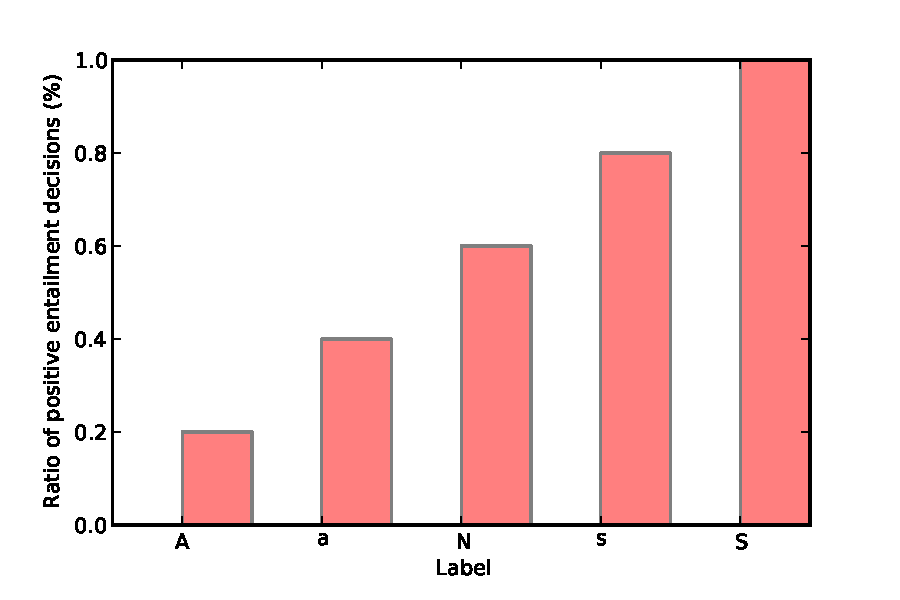
\includegraphics{entailment.pdf}
\caption{Ratio of positive entailment decisions across labels, scaled to a $[0,1]$ interval
}
\label{fig:entailment_ratio}
\end{figure}

% entailment
- Following the work of \citet{cabrio2012combining}, we use textual 
entailment to determine whether the comment (text) entails the prominent
claim (hypothesis) \\
- to this end, we use the Excitement Open Platform (EOP)
\citep{pado2015design} \\
- from EOP, we used seven pre-trained \textit{entailment decision algorithms}
(EDAs) \\
- some EDAs use only syntactical features, whereas others rely on
WordNet \citep{miller1995wordnet}, VerbOcean \citep{chklovski2004verbocean} \\
- each EDA outputs a binary decision (\textit{Entailment} or \textit{NonEntailment})
along with a degree of confidence \\
- we use all seven (decisions and confidences) of EDAs as features for our classifier 
(14 features in total) \\
- we experiment with additional features (the disjunction of all classifier decisions, 
max of seven EDA confidence values, mean value of seven EDA confidences), but those
did not impact performance \\
- the motivation for this set of features is that we expect the comment text (usually longer and specific)
to entail the prominent claim (usually shorter and more general) \\
- this intuition is confirmed in figure~\ref{fig:entailment_ratio}
where it shown that 
pro prominent claims have a higher ratio of positive entailment decisions than con prominent claims \\
- also vaguely supported prominent claims have a lower rate of entailment
decisions than explicitly supported prominent claims \\

% semantic textual similarity
- the prominent claim should either be entailed or not entailed from the comment \\
- the former case includes a paraphrase \\
- in the latter case, there might be a contradiction or it may be \textit{non sequitur} \\
- these relations can be hard to detect, especially from vaguely stated comments \\
- to account for this, we use a feature based on semantic textual similarity (STS) \\
- we use TakeLab's STS \citep{vsaric2012takelab} which works as described in
section~\ref{sec:sts} \\


\section{Experimental Evaluation}
\label{sec:argrec_experiments}

\section{Conclusion}
\label{sec:argrec_conclusion}
